\chapter{Results}
\label{results}

In this chapter, we present the results of the anomaly detection experiments carried out on two different feature embeddings. We use two methods of evaluation: comparison of accuracy, precision, recall and $F1$ metrics to evaluate the performance using the labeled test dataset and dual validation of the results with the help of domain experts.

%https://researchbank.swinburne.edu.au/file/cee84793-6f09-49ce-a099-41451c803b81/1/mostafa_farshchi_thesis.pdf page 120 evaluation

Proper evaluation is a crucial step in machine learning. In supervised techniques, it is usually checked how is the model performing on the training data, but also on previously unseen datasets called \textit{test} or \textit{validation} data sets using various performance metrics. If the results are unsatisfactory, this information can be used to tweak model hyperparameters and repeat the process. However, in case of unsupervised learning that we have employed in our research, it is not immediately obvious how to approach model evaluation. 

The only dataset we may consider labeled is the Nightly dataset used for training. All data collected during the night are \textit{normal} instances without anomalies, but we need to test whether the actual anomalies are being recognized by our detectors and whether the detected anomalies correspond with actual anomalies. 

As we have described in Chapter \ref{chapter:dataset} when defining our datasets, we have manually created a testing set of logs that contains two types of observed anomaly scenarios included in Anomalies dataset: Killing the Redis server and Killing the RabbitMQ message broker. In our simulations of these scenarios, we know specific time range when an anomaly occurs, therefore we are able to label specific feature embeddings by hand. Moreover, a fraction of Nightly Test dataset that contains data not seen during the training phase is also used as a part of the testing dataset. Lastly, we include the Call dataset into our test set containing a set of log messages generated during calls, as it is very important that our models do not recognize calls as anomalies.

The weakness of this approach is that there are only two known types of anomalies in the testing dataset. There is no way to tell if the models behave correctly on live, production data. As a compromise, we will us a Daily dataset, whose labels are unknown, to generate predictions. After that, we carry out a so called \textit{expert validation}. We ask the domain experts at Motorola Solutions SmartConnect's team to evaluate a small subset of predictions generated by our best-performing models. 


\section{Test Dataset Validation}

Anomaly detection models interpreted through the evaluation metrics obtained on the testing set (Section \ref{section:testset}) containing two types of anomalies helped us verify \textbf{RQ1} proposed in Chapter \ref{introduction}, that the logs produced by Motorola Smart Connect are indeed generated in a way that they can be used for anomaly detection. Let's take a closer look at the results of the machine learning algorithms, which enable us to answer the rest of the research questions.

Table \ref{tab:results} gives the summarized experiment results on testing dataset for Isolation Forest, PCA, Invariants Mining and Log Clustering models. We will first compare the results in terms of feature embeddings and then we will discuss how did the different anomaly detection algorithms perform relatively to each other. 

\begin{table}[h]
\centering
\resizebox{\textwidth}{!}{\begin{tabular}{@{}cccccc@{}}
\toprule
\textbf{Algorithm}         & \textbf{Embedding}                                           & \textbf{Precision}                                         & \textbf{Recall}                                             & \textbf{F1}                                                 & \textbf{Accuracy}                                           \\ \midrule
\textcolor{customGreen}{\textbf{Isolation Forest}}  & \begin{tabular}[c]{@{}c@{}}Event count\\ TF-IDF\end{tabular} & \begin{tabular}[c]{@{}c@{}}100.00\%\\ 33.33\%\end{tabular}  & \begin{tabular}[c]{@{}c@{}}57.14\%\\ 14.81\%\end{tabular}   & \begin{tabular}[c]{@{}c@{}}66.67\%\\ 20.51\%\end{tabular}    & \begin{tabular}[c]{@{}c@{}}87.79\%\\ 76.15\%\end{tabular}    \\ \midrule
\textcolor{customGreen}{\textbf{PCA}}               & \begin{tabular}[c]{@{}c@{}}Event count \\ TF-IDF\end{tabular} & \begin{tabular}[c]{@{}c@{}}100.00\%\\ 100.00\%\end{tabular} & \begin{tabular}[c]{@{}c@{}}100.00\%\\ 100.00\%\end{tabular} & \begin{tabular}[c]{@{}c@{}}100.00\%\\ 100.00\%\end{tabular}  & \begin{tabular}[c]{@{}c@{}}100.00\%\\ 100.00\%\end{tabular}  \\ \midrule
\textcolor{customGreen}{\textbf{Invariants Mining}} & \begin{tabular}[c]{@{}c@{}}Event count\\ TF-IDF\end{tabular} & \begin{tabular}[c]{@{}c@{}}22.22\%\\ 21.60\%\end{tabular}   & \begin{tabular}[c]{@{}c@{}}100.00\%\\ 100.00\%\end{tabular}  & \begin{tabular}[c]{@{}c@{}}36.36\%\\ 35.53\%\end{tabular}    & \begin{tabular}[c]{@{}c@{}}25.19\%\\ 24.62\%\end{tabular}    \\ \midrule
\textcolor{customGreen}{\textbf{Log Clustering}}    & \begin{tabular}[c]{@{}c@{}}Event count\\ TF-IDF\end{tabular} & \begin{tabular}[c]{@{}c@{}} 100.00\%\\  100.00\%\end{tabular}          & \begin{tabular}[c]{@{}c@{}}100.00\%\\ 100.00\%\end{tabular} & \begin{tabular}[c]{@{}c@{}}100.00\%\\ 100.00\%\end{tabular} & \begin{tabular}[c]{@{}c@{}}100.00\%\\ 100.00\%\end{tabular} \\ \bottomrule
\end{tabular}}
 \caption{The precision, recall, F1 score and accuracy for anomaly detection detection methods calculated on testing dataset on two different embeddings: event count and TF-IDF. Both embeddings are generated using a two minute sliding window.}
    \label{tab:results}
\end{table}


\subsection{Feature Embeddings Comparison}
To address \textbf{RQ2} we wanted to see how do different feature embeddings into a numerical vectors effect the results. As described in previous chapters, we proposed two embeddings: Simple event count vector and weighted TF-IDF vector. TF-IDF is obtained from event count weight by adding more weight to the events that are happening less frequently in the whole dataset. We were interested to see if this kind of information can bring any more information that would be beneficial for the anomaly detection model.

It is clear from the results that both embeddings performed very similarly and from the testing dataset, it is impossible to tell which one would do better on unknown anomalies. If we look at Figure \ref{fig:tf-vs-tfidf} comparing the t-SNE visualization applied on normal datapoints and anomaly datapoints of different embeddings, we can see that both event count and TF-IDF dealt with anomalies and normal data in similar fashion. Both event count embedding and TF-IDF embedding produced clusters in the embedding space that are visually visible and are able to distinguish between normal and anomalous data points.

Another means of comparison of these two embeddings is by observing the histogram provided in Figure \ref{fig:histogram-event-types}. We expected TF-IDF to assign a higher value to the events that occur rarely, which should by our assumption include events that are representative for anomalies. Histogram seem to be in align in the middle part of the plot, but a significantly lower weight is observed for the first five hundred event type IDS in TF-IDF histogram in comparison with event count histogram. After inspecting the feature vectors manually, we have noticed a pattern in the frequency of event types with lower IDs. The respective event types are appearing in consecutive log sequences in identical frequencies. This is expected and reasonable, as events behind these event type IDs include starting a call, attempting to start a new TLS connection and other regularly appearing events. Thus, these event type can be consider as frequently occuring, therefore they are being assigned lower weight by TF-IDF algorithm which is reflected by the histogram.

All in all, if we take account that event count embbedding is simple and much easier to interpret than TF-IDF and TF-IDF did not perform significantly better on the testing dataset, we consider event count embedding being a preferred representation of the dataset for practical use.

% Distribution graph to compare the TF IDF to see how many TFIDF had high occurency


\begin{figure}[h]%
    \centering
    \subfloat[\centering Event count embedding]{{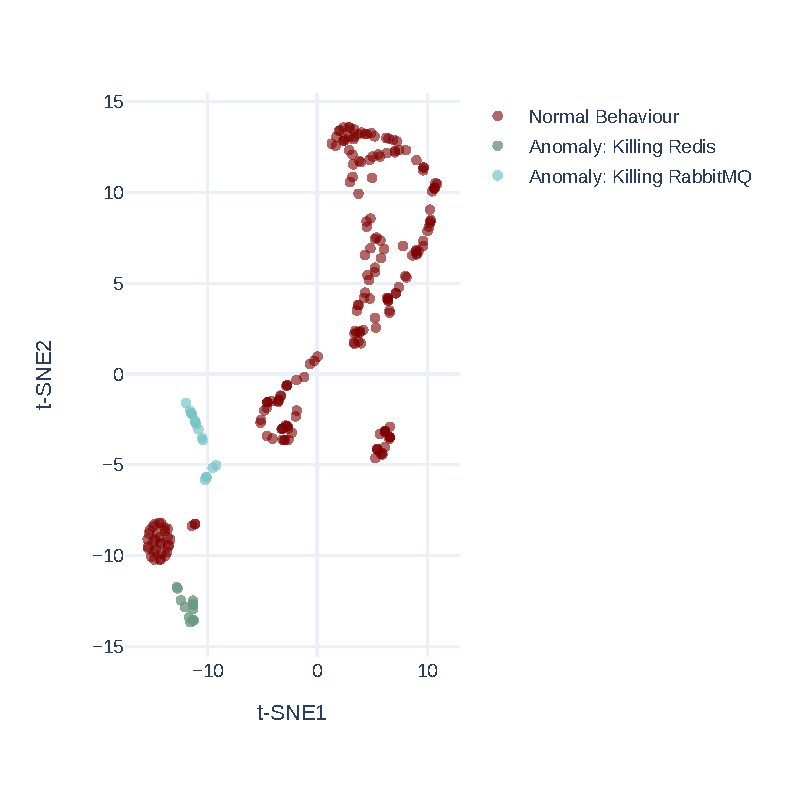
\includegraphics[width=5.52cm]{img/tsne-anomalies-vs-normal-small.pdf} }}%
    \qquad
    \subfloat[\centering TF-IDF embedding]{{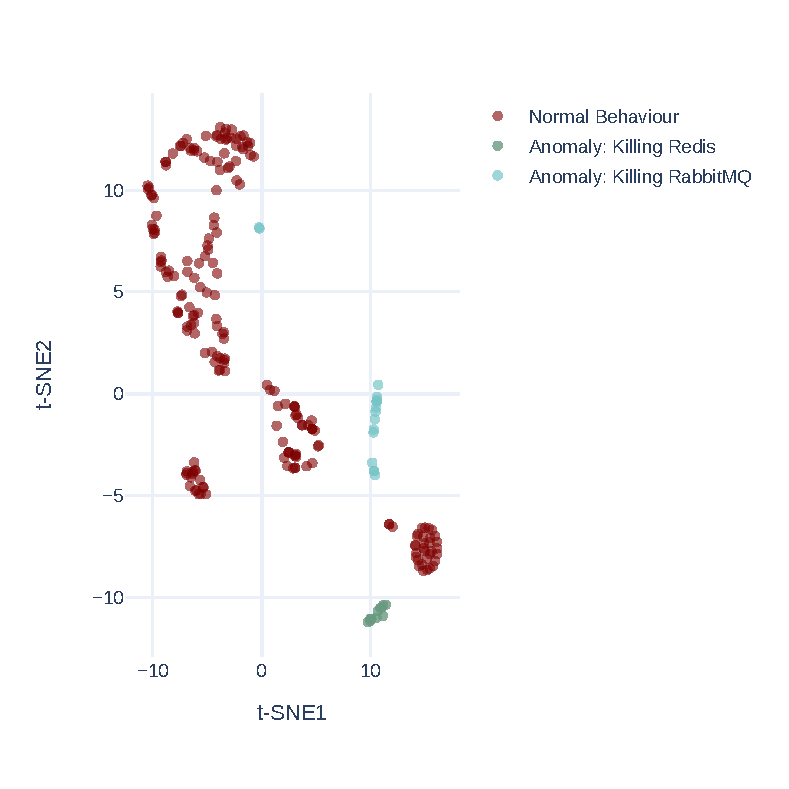
\includegraphics[width=5.52cm]{img/tsne-anomalies-vs-normal-tfidf.pdf} }}%
    \caption{Event count embedding (left) and TF-IDF embedding (right) of the normal and anomalous log sequences plotted using PCA.}%
    \label{fig:tf-vs-tfidf}%
\end{figure}

\begin{figure}[h]%
    \centering
    \subfloat[\centering Event count]{{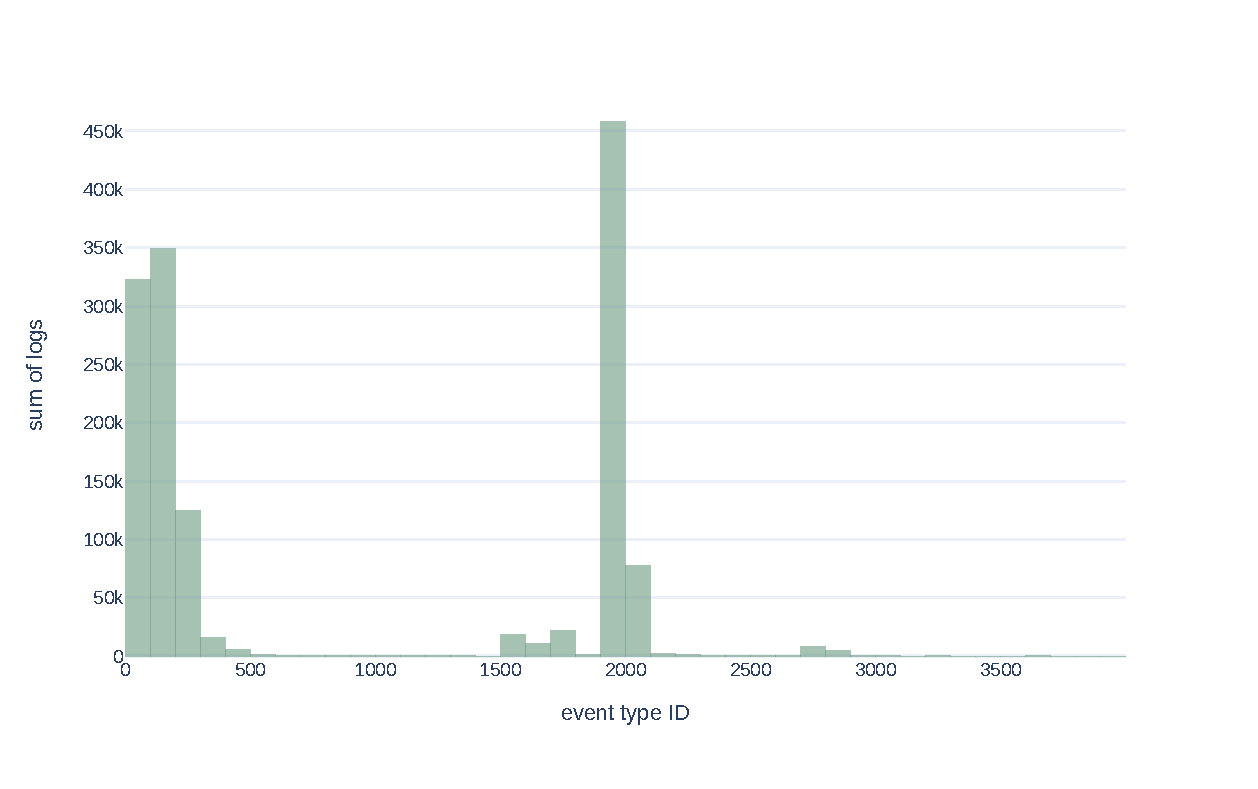
\includegraphics[width=0.9\textwidth]{img/tf-histogram.pdf} }}%
    \qquad
    \subfloat[\centering TF-IDF]{{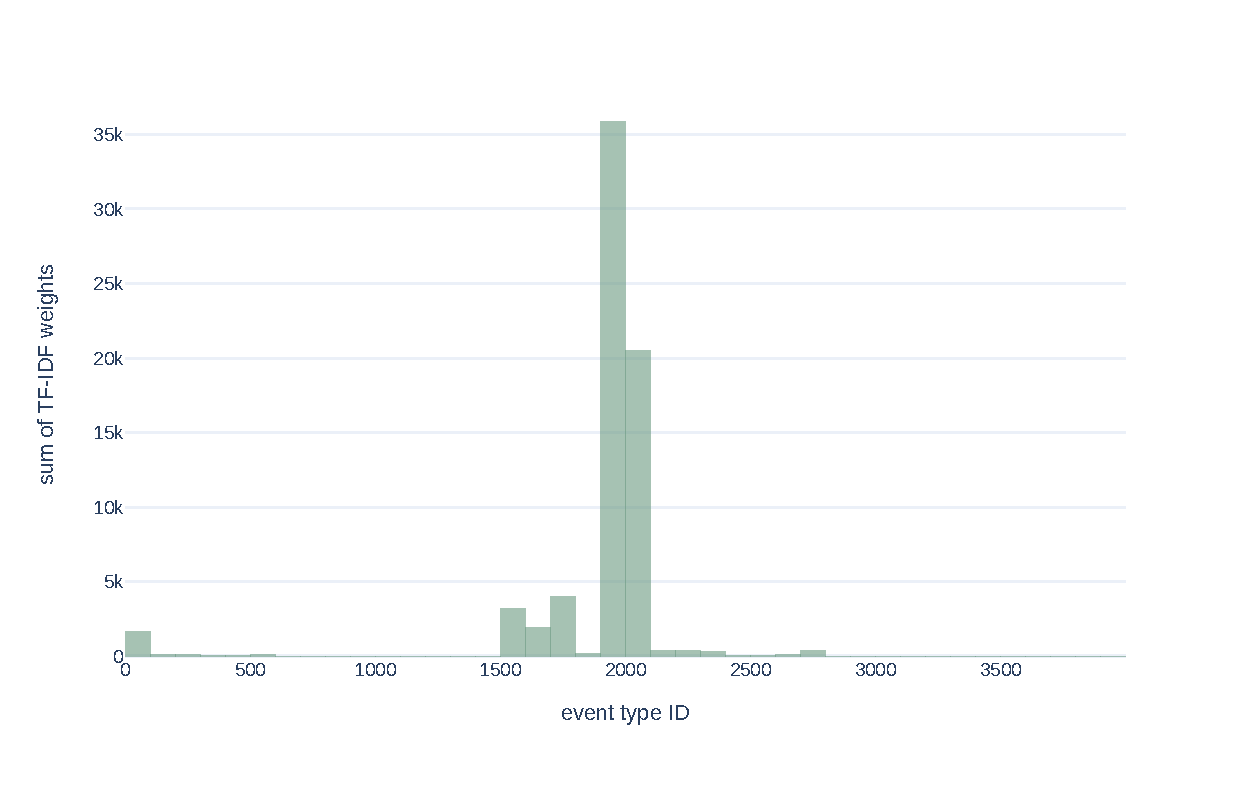
\includegraphics[width=0.9\textwidth]{img/tfidf-histogram.pdf} }}%
    \caption{Histogram distribution plot of event type IDs in testing dataset, where the logs of same the same event type ID represented yb x-axis are binned together and their cumulative counts are represented by the y-axis. (a) is a histogram of generated over event count embeddings and (b) is a histogram generated over TF-IDF embeddings.}%
    \label{fig:histogram-event-types}%
\end{figure}


\subsection{Anomaly Detection Methods Comparison}
In this section we will describe how well do the four proposed anomaly detection methods perform on the labeled testing dataset. To support our reasonings, we will refer to the reported experiment results using evaluation metrics on \textit{event count} embedding of testing dataset with a two minute sliding window from Table \ref{tab:results}. 

In order of importance, for a live production system it is more important not to miss an anomaly rather than correctly detect anomaly-free data points. In other words, false negatives are more alarming than false positives. To analyze the ratio of identified anomalous and non-anomalous log sequences within all dataset, we derived derive confusion matrices for Isolation Forest, PCA, Invariants Mining and Log Clustering models respectively in Table \ref{table:confusionMatrix:if}, Table \ref{table:confusionMatrix:pca}, Table \ref{table:confusionMatrix:im} and Table \ref{table:confusionMatrix:clustering}. Figure \ref{fig:tsne-predictions-labeled} gives a visual interpretation of which points got misclassified in each anomaly detection method. 

From the table of results we can see that all the anomaly detection methods produce decent result, 
whereas Log Clustering and PCA clearly outperformed Invariants Mining and Isolation Forest. 

Among the four unsupervised anomaly detection algorithms, evaluation metrics are the lowest for Invariants Mining model with the values of $22.22\%$ precision, $100.00\%$ recall and $36.36\%$ F1 score. Figure \ref{fig:tsne-predictions-labeled} (c) shows that Invariants Mining has a tendency to falsely recognize normal data points as anomalies. Its poor perfomance did not come as a surprise and we suspect there are two reasons for this occurence. Firstly, as we explained in Section \ref{section:experimental-setup}, we did not perform hyperparameter exploration, as the training process for Invariants Mining is extremely ineffective on our dataset. However, we assume that the main reason for its inability to detect anomalies stems from how we performed windowing into log sequences. In similar research papers that successfully employed Invariants Mining, such as He et al. \cite{he2016}, they used \textit{session ID} or \textit{process ID} shared among logs as a key of grouping logs into log sequence. On the flip side, we have focused on the timely relationship between logs and grouped them into log sequences in successive two minutes windows. As a result, it is not guaranteed that log events that are part of invariants uncovered by Invariants Mining will be in the same log sequence in the resulting embedding. Thus, it is expected for Invariants Mining method not to perform well on our log dataset feature representation.

Another algorithm that did not obtain good results is Isolation Forest with $100.00\%$ precision, but $57.14\%$ recall and $66.67\%$ F1 score. In \ref{fig:tsne-predictions-labeled} (a) we can observe Isolation Forest misses a high number of anomalies yielding a low recall and a high number of false negatives, as well as false positives \todo{check}. We concluded that a reason for this finding is that Isolation Forest is not well suited for one-class learning case (training set containing only negative samples) \cite{adForest}. The leaves of iTrees provide an anomaly score, that corresponds to the length of the average path from the node (sample from training set) to that leaf. The shorter the path, the smaller the anomaly score and the higher probability that it is an outlier. Since all samples in the training dataset are normal, assigned anomaly scores might be biased. Thus, Isolation Forest does not perform well on our dataset.

Log Clustering and PCA achieved superior performance comparing to other anomaly detection methods proposed in our research. The final result is $100.00\%$ precision, recall, F1 score and accuracy on the testing dataset for both Log Clustering and PCA. It is of our interest to further investigate these two algorithms and in the next section, we will ask developers at Motorola Solutions to evaluate the results of these two algorithms on a previously unseen dataset (Daily), for which we do not have any labels and only experts who know the field can tell if the predictions are correct. 

\begin{figure}%
    \centering
    \subfloat[\centering Isolation Forest]{{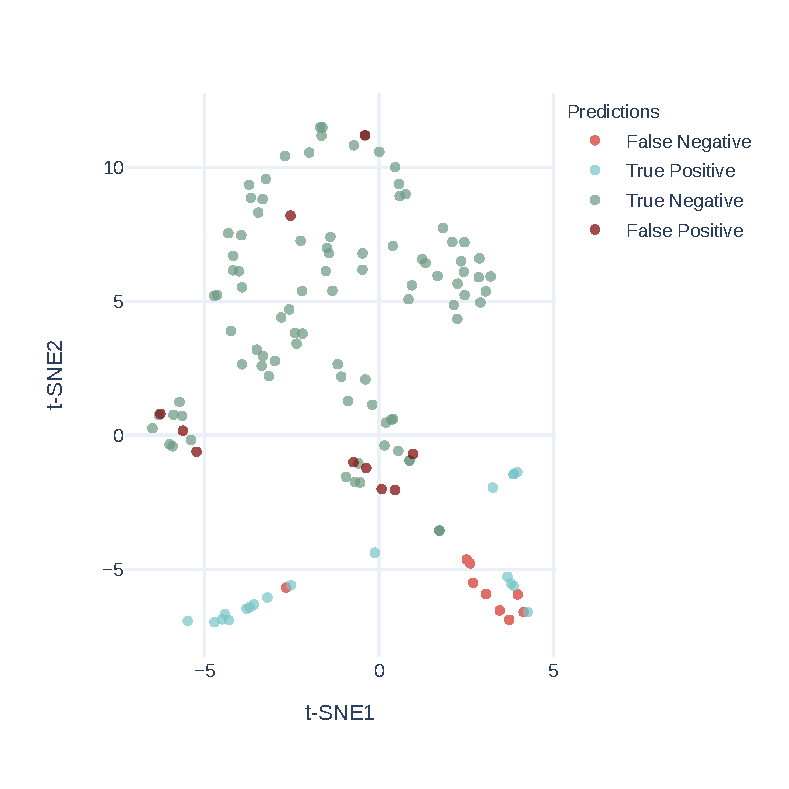
\includegraphics[width=5.52cm]{img/tsne-predictions-isolation-forest.pdf} }}%
    \qquad
    \subfloat[\centering PCA]{{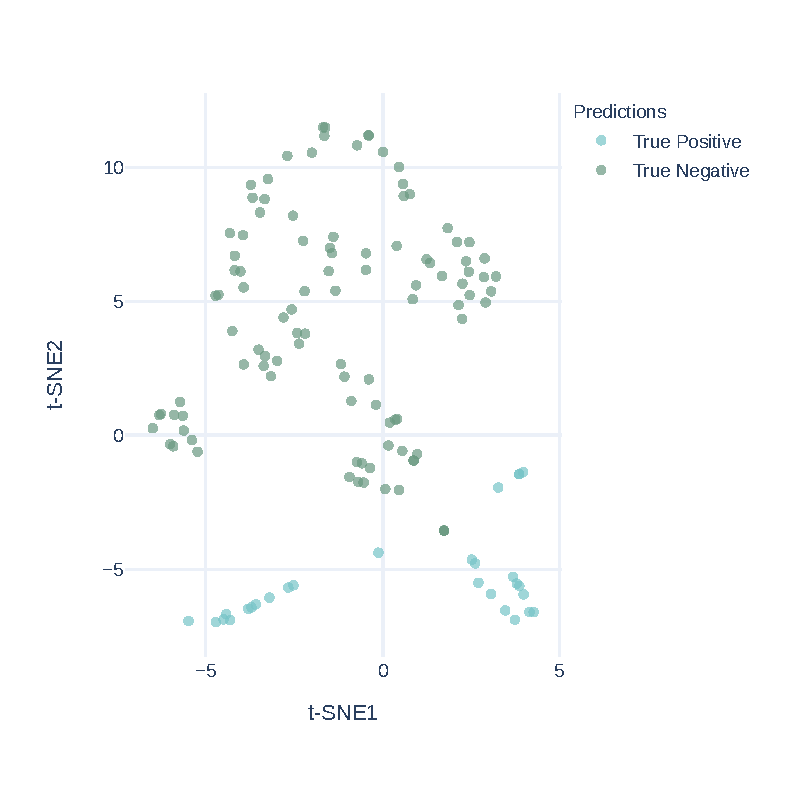
\includegraphics[width=5.52cm]{img/tsne-predictions-pca.pdf} }}%
    \qquad
    \subfloat[\centering Invariants Mining]{{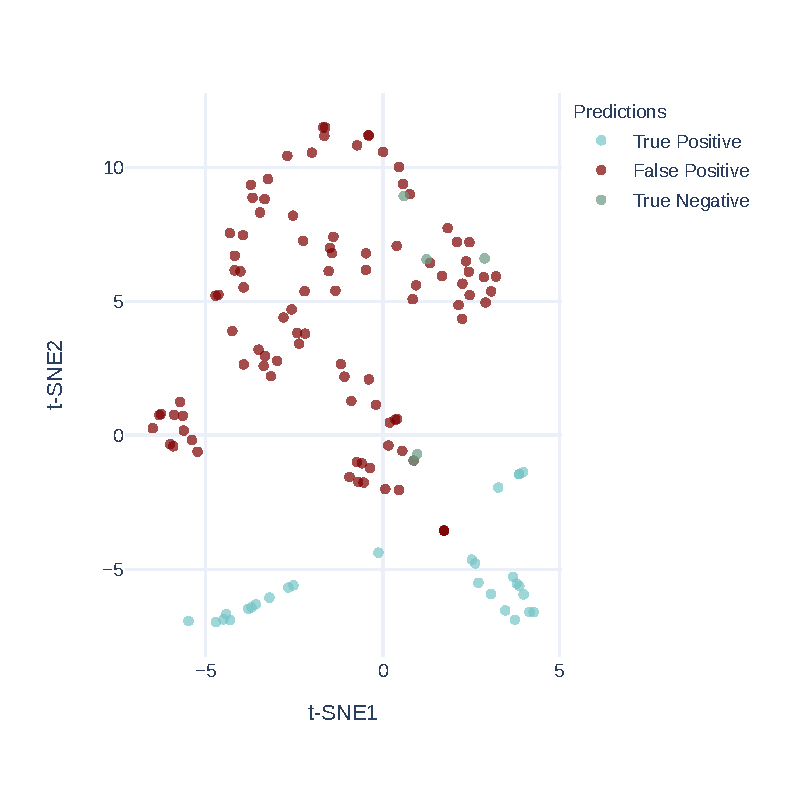
\includegraphics[width=5.52cm]{img/tsne-predictions-invariants-mining.pdf} }}%
    \qquad
    \subfloat[\centering Log Clustering]{{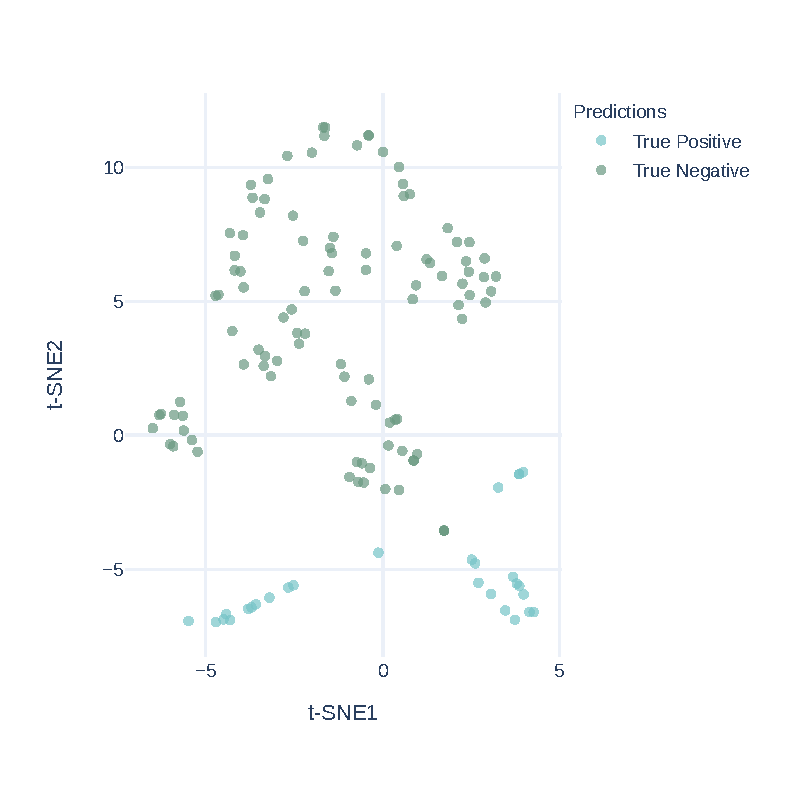
\includegraphics[width=5.52cm]{img/tsne-predictions-clustering.pdf} }}%
    \caption{Comparison of Isolation Forest (a), PCA (b), Invariants Mining (c) and Log Clustering (d) predictions on the labeled testing dataset. It can be observed from the plots that PCA and Log Clustering algorithms handle testing dataset with a $100 \%$ accuracy.}%
    \label{fig:tsne-predictions-labeled}%
\end{figure}


\begin{table}[!h]
\centering
\begin{tabular}{cccc}
\multicolumn{1}{r}{}                 &                              & \textbf{Predicted}          &   $\hat{l}$                          \\ \cline{3-4} 
                                     & \multicolumn{1}{l|}{}        & \multicolumn{1}{l|}{Anomaly} & \multicolumn{1}{l|}{Normal} \\ \cline{2-4} 
                                      
\multicolumn{1}{l|}{\textbf{Actual}} & \multicolumn{1}{l|}{Anomaly}  & \multicolumn{1}{l|}{\textcolor{customBlue}{\textbf{19}}}     & \multicolumn{1}{l|}{\textcolor{customRed}{\textbf{9}}}      \\ \cline{2-4} 
\multicolumn{1}{c|}{\textit{l}}                & \multicolumn{1}{c|}{Normal} & \multicolumn{1}{l|}{\textcolor{customDarkRed}{\textbf{10}}}     & \multicolumn{1}{l|}{\textcolor{customGreen}{\textbf{93}}}      \\ \cline{2-4} 
\end{tabular}
\caption{A confusion matrix for Isolation Forest model on testing dataset.}
\label{table:confusionMatrix:if}
\end{table}


\begin{table}[!h]
\centering
\begin{tabular}{cccc}
\multicolumn{1}{r}{}                 &                              & \textbf{Predicted}          &   $\hat{l}$                          \\ \cline{3-4} 
                                     & \multicolumn{1}{l|}{}        & \multicolumn{1}{l|}{Anomaly} & \multicolumn{1}{l|}{Normal} \\ \cline{2-4} 
                                      
\multicolumn{1}{l|}{\textbf{Actual}} & \multicolumn{1}{l|}{Anomaly}  & \multicolumn{1}{l|}{\textcolor{customBlue}{\textbf{28}}}     & \multicolumn{1}{l|}{\textcolor{customRed}{\textbf{0}}}      \\ \cline{2-4} 
\multicolumn{1}{c|}{\textit{l}}                & \multicolumn{1}{c|}{Normal} & \multicolumn{1}{l|}{\textcolor{customDarkRed}{\textbf{0}}}     & \multicolumn{1}{l|}{\textcolor{customGreen}{\textbf{103}}}      \\ \cline{2-4} 
\end{tabular}
\caption{A confusion matrix for PCA model on testing dataset.}
\label{table:confusionMatrix:pca}
\end{table}


\begin{table}[!h]
\centering
\begin{tabular}{cccc}
\multicolumn{1}{r}{}                 &                              & \textbf{Predicted}          &   $\hat{l}$                          \\ \cline{3-4} 
                                     & \multicolumn{1}{l|}{}        & \multicolumn{1}{l|}{Anomaly} & \multicolumn{1}{l|}{Normal} \\ \cline{2-4} 
                                      
\multicolumn{1}{l|}{\textbf{Actual}} & \multicolumn{1}{l|}{Anomaly}  & \multicolumn{1}{l|}{\textcolor{customBlue}{\textbf{28}}}     & \multicolumn{1}{l|}{\textcolor{customRed}{\textbf{0}}}      \\ \cline{2-4} 
\multicolumn{1}{c|}{\textit{l}}                & \multicolumn{1}{c|}{Normal} & \multicolumn{1}{l|}{\textcolor{customDarkRed}{\textbf{98}}}     & \multicolumn{1}{l|}{\textcolor{customGreen}{\textbf{5}}}      \\ \cline{2-4} 
\end{tabular}
\caption{A confusion matrix for Invariants Mining model on testing dataset.}
\label{table:confusionMatrix:im}
\end{table}

\begin{table}[!h]
\centering
\begin{tabular}{cccc}
\multicolumn{1}{r}{}                 &                              & \textbf{Predicted}          &   $\hat{l}$                          \\ \cline{3-4} 
                                     & \multicolumn{1}{l|}{}        & \multicolumn{1}{l|}{Anomaly} & \multicolumn{1}{l|}{Normal} \\ \cline{2-4} 
                                      
\multicolumn{1}{l|}{\textbf{Actual}} & \multicolumn{1}{l|}{Anomaly}  & \multicolumn{1}{l|}{\textcolor{customBlue}{\textbf{28}}}     & \multicolumn{1}{l|}{\textcolor{customRed}{\textbf{0}}}      \\ \cline{2-4} 
\multicolumn{1}{c|}{\textit{l}}                & \multicolumn{1}{c|}{Normal} & \multicolumn{1}{l|}{\textcolor{customDarkRed}{\textbf{0}}}     & \multicolumn{1}{l|}{\textcolor{customGreen}{\textbf{103}}}      \\ \cline{2-4} 
\end{tabular}
\caption{A confusion matrix for Log Clustering model on testing dataset.}
\label{table:confusionMatrix:clustering}
\end{table}


\section{Expert Validation}

Thanks to the developers at Motorola Solutions, we were able to obtain an external validation of our results. We consulted experts to evaluate the discovered anomalies, as well to evaluate samples that were recognized as normal by two of the best performing anomaly detection models: PCA and Log Clustering.

In Figure \ref{fig:tsne-unlabeled-plots} are shown the t-SNE plots of the predictions on Daily data obtained from the trained PCA and Log Clustering models. For t-SNE and PCA plots generated on the predictions of Daily dataset by the rest of the less performing algorithms studied in our research, see Appendix \ref{fig:tsne-unlabeled-plots-appendix} and Appendix \ref{fig:pca-unlabeled-plots-appendix} respectively. 
\begin{figure}%
    \centering
    \subfloat[\centering Log Clustering]{{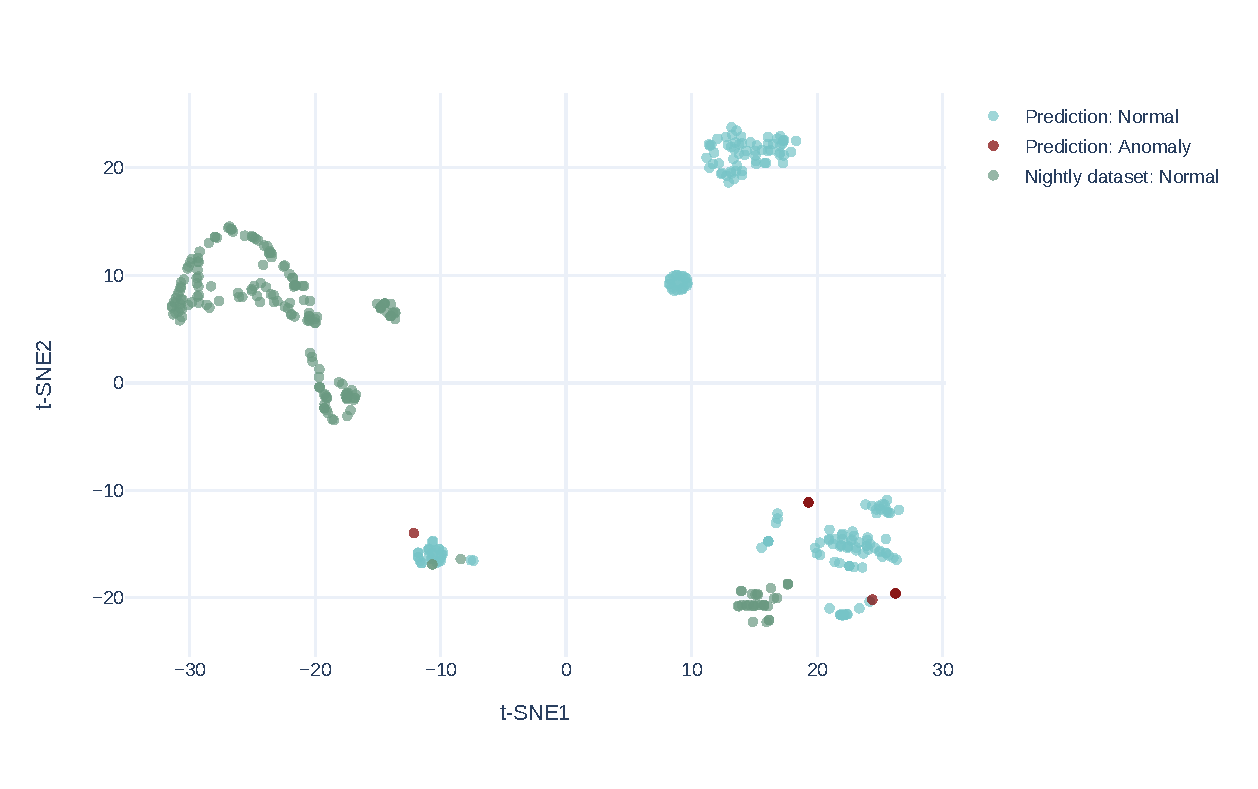
\includegraphics[width=0.9\textwidth]{img/tsne-predictions-unlabeled-clustering.pdf} }}%
    \qquad
    \subfloat[\centering PCA]{{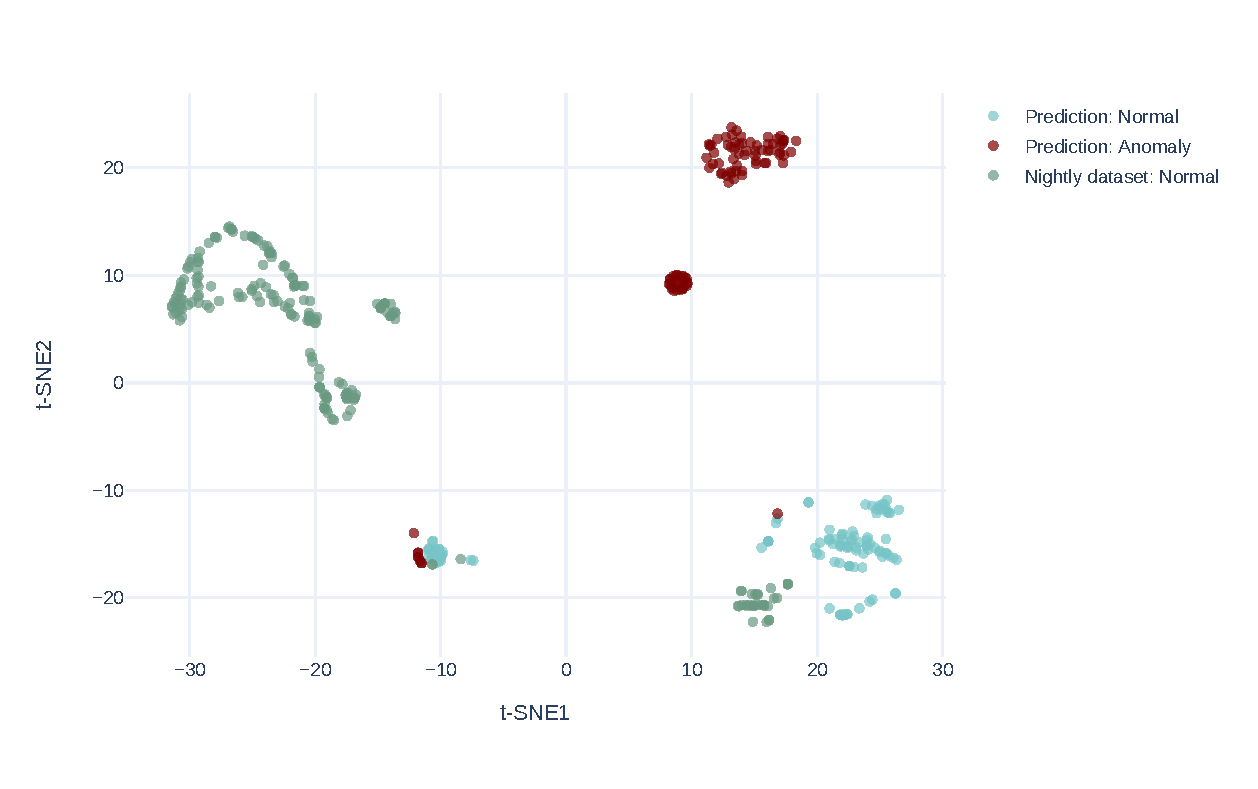
\includegraphics[width=0.9\textwidth]{img/tsne-predictions-unlabeled-pca.pdf} }}%
    \caption{Comparison of Log Clustering (left) and PCA (right) predictions on the unlabeled Daily dataset. Green data points represent the normal datapoints as a point of reference, data points highlighted in blue and red represent predictions of normal or anomalous log sequence respectively.}%
    \label{fig:tsne-unlabeled-plots}%
\end{figure}

\subsection{Analysis}
The goal of this step was to confront our machine learning models with anomalies that are difficult to simulate manually or are unknown, and therefore we were not able to validate against them on a larger scale. However, since our models are designed to be able to identify previously unseen anomalies, we studied a random sample from experimental environment during the day. It should follow a very different distribution comparing to both the nightly dataset and the dataset with known anomalies.

The experts were given a small sample of time windows extracted from the Daily dataset. The sample of \todo{how many} windows was given to them in form of both \textit{histogram} of event templates and a sequence of \textit{raw logs}. The specific time windows were chosen based on its predicted label, such that each predicted class had several representative windows in the sample for both of the best performing anomaly detection models, Log Clustering and PCA. We tried to choose time windows, who's predicted labeled differed among the models, as well as those that were the same.

In these windows, the domain experts managed to identify an anomaly, where UDP packets information are being dropped. The packets usually carry the audio information of the calls and their loss may be caused by poor connectivity which as a result may decrease the overall quality of send or received calls.  This is certainly a valid anomaly that is desired to be detected. 

After further inspection we noticed that the cluster in the top right corner corresponds with the anomaly of a dropped packet. As can be observed in Figure~\label{fig:tsne-unslabeled-plots}, this behaviour was only recognized as an anomaly by PCA. On the other hand, Log Clustering is less sensitive towards the cluster which contains calls with bigger pocket loss. If this specific anomaly happens, it doesn't trigger more processes in the system and it continues running as usual, trying to deliver them on basis of the best-effort delivery, therefore it can be also argued that if UDP dropout of small size is not an anomaly that needs to raise alarms. The fact that Log Clustering did not recognize these points as anomalies could be resolved be adjusting hyperparameters.

On the other hand, the experts did not report any false negatives (anomalies labelled as anomaly free by our models). This information on its own however doesn't prove that there are no instances of those.
Clearly, it is more difficult to identify a false positive by hand as in general there would be many more windows labeled as anomaly-free and we cannot expect human to crawl through all of them effectively verifying that no false negative occurred in the analyzed time span. It is understandable that a bare eye is not able to spot these just based on the histogram and logs assigned to each of the windows that are meant for troubleshooting the predictions.